%---------------------------------------------------------------
\chapter{Implementace serveru}
%---------------------------------------------------------------

\begin{chapterabstract}
    V této kapitole popíšu průběh implementace serveru, jednotlivé třídy a zajímavosti, se kterými jsem se při implementaci setkal.
\end{chapterabstract}

\section{Úvod}

Pro implementaci serveru jsem se rozhodl využít technologii Spring Web \cite{spring-web} v programovacím jazyce Kotlin \cite{kotlin}. Nad touto technologií jsem postavil vlastní nadstavbu, která s pomocí šablon generuje velkou část obecného kódu pro zpřístupnění dat s pomocí REST API. Implementace těchto základních CRUD (z anglického Create = vytvoření, Read = čtení, Update = úprava, Delete = smazání) operací je tak velmi rychlá a spočívá především v definici dat v databázi (datová vrstva, balíček Entity), definici tříd pro přenos dat mezi business a prezentační vrstvou (business vrstva, balíček DTO) a definici oprávnění pro jednotlivé operace (prezentační vrstva, balíček Controller).

\section{Datová vrstva}

Datová vrstva se skládá ze dvou balíčků, Entity a Repository. Tato vrstva je obstarána frameworkem Spring JPA \cite{spring-jpa}. Pro zpřístupnění základních CRUD operací jsem tedy pouze vytvořil rozhraní Repository s danou Entitou jako parametrem šablony, konkrétní implementaci včetně komunikace s databází vygeneroval framework.

\subsection{Entity}

Entity jsou reprezentovány jako datové třídy v Kotlinu. Každá entita reprezentuje jednu tabulku v relační databázi a pomocí anotací u proměnných definuji jednotlivé sloupce těchto tabulek včetně integritních omezení a cizích klíčů (vazeb s ostatními entitami). Entity, se kterými pracuji, jsou uživatel (User), zpěvník (SongBook), píseň (Song), poznámka (SongNote), kapela (Band), role (Role) a členství v kapele (BandMember).

Každá entita obsahuje unikátní identifikátor, který je primárním klíčem v databázi a metody \texttt{canView} (může vidět) a \texttt{canEdit} (může upravit), které určují, zda má daný uživatel přístup k~dané entitě.

\begin{listing}
\begin{minted}[breaklines,breaksymbolleft=]{kotlin}
@Entity
@Table (uniqueConstraints=[UniqueConstraint(columnNames = ["name", "band_id"])])
data class SongBook (
    @Column(nullable = false) val name: String,
    @OneToMany(mappedBy = "songBook")
    val songs: List<Song>,

    @ManyToOne
    @JoinColumn (name = "band_id", nullable = false)
    val band: Band,
    override val id: Int = 0
) : IEntity(id) {
    override fun canEdit (user: User)
        = user.bands.any { it.role.level == RoleLevel.LEADER && it.band.id == band.id }
    override fun canView (user: User?)
        = user?.bands?.any { it.band.id == band.id } ?: false
}
\end{minted}
\caption[Ukázka třídy pro zpěvník]{Ukázka třídy pro zpěvník (SongBook). V definici lze vidět integritní omezení -- unikátní klíč na sloupcích jméno a identifikátor kapely, textový sloupec pro jméno, definici 1:N vazby s entitou píseň (Song), M:1 vazby s entitou kapela (Band), kde bude spojení provedeno přes sloupec band\_id a metody \texttt{canEdit} a \texttt{canView}, které umožní uživateli zpěvník upravit/zobrazit, pokud je vedoucím/členem kapely, v níž je aktuální zpěvník}
\end{listing}

\subsection{Repository}

Repository jsou ve Spring JPA definovány pouze jako rozhraní. Metody pro základní CRUD operace jsou vygenerovány frameworkem a není je třeba zvlášť definovat. Pro hledání podle jiných kritérií než je identifikátor entity -- například hledání zpěvníků podle kapel, písní podle zpěvníků nebo poznámek podle uživatele je nezbytné definovat novou metodu (implementaci vygeneruje JPA) s pomocí anotace \texttt{@Query} a dotazu napsaného v dotazovacím jazyce JPQL (Jakarta Persistence Query Language) \cite{jpql}.

\begin{listing}[H]
\begin{minted}[breaklines,breaksymbolleft=]{kotlin}
@Repository
interface SongBookRepository : IRepository<SongBook> {
    @Query("SELECT sb FROM SongBook sb WHERE sb.band IN :bands")
    fun findByBands(bands: List<Band>) : List<SongBook>
}
\end{minted}
\caption[Ukázka třídy Repository pro zpěvník]{Ukázka třídy SongBookRepository s metodou pro hledání zpěvníků podle kapel}
\end{listing}

\section{Business vrstva}

Business vrstva se skládá ze dvou balíčků, Service a DTO. Cílem business vrstvy je zprostředkovat data z datové vrstvy a odpovědět s jejich pomocí na dotazy z prezentační vrstvy. Tato vrstva je částečně obstarána mou nadstavbou, pro zpřístupnění základních CRUD operací tak stačí vytvořit třídu Service, která dědí z abstraktní šablony \texttt{IServiceImpl} s danou entitou a DTO jako parametry této šablony.

\subsection{DTO}

DTO (z anglického data transfer object) jsou speciální datové třídy, které slouží ke komunikaci mezi business a prezentační vrstvou. Existují DTO tří typů -- DTO ke čtení (\texttt{IReadDTO}), k~úpravě (\texttt{IUpdateDTO}) a k vytvoření (\texttt{ICreateDTO}). Každé \texttt{IReadDTO} musí obsahovat identifikátor entity a slouží k zprostředkování dat \textbf{z databáze} směrem k prezentační vrstvě. \texttt{ICreateDTO} a \texttt{IUpdateDTO} slouží k vytváření a úpravě entity a zprostředkovávají data z prezentační vrstvy směrem \textbf{do~databáze}. Rozdíl mezi \texttt{ICreateDTO} a \texttt{IUpdateDTO} je pak ten, že \texttt{IUpdateDTO} má nepovinné parametry -- parametry, které budou vynechány, nebudou aktualizovány.

\begin{listing}[H]
\begin{minted}[breaklines,breaksymbolleft=]{kotlin}
data class SongBookReadDTO (override val id: Int, val name: String, val band: BandReadDTO, val songs: List<SongReadDTO>) : IReadDTO
data class SongBookUpdateDTO (val name: String?, val bandId: Int?) : IUpdateDTO
data class SongBookCreateDTO (val name: String, val bandId: Int) : ICreateDTO
\end{minted}
\caption[Ukázka DTO tříd pro zpěvník]{Ukázka souboru s DTO třídami pro zpěvník (SongBookDTO). Při čtení se zde vrací jméno zpěvníku, DTO popisující kapelu a seznam písní ve zpěvníku. Při vytváření/úpravě zpěvníku se používá jméno a identifikátor kapely, zpěvník se vytvoří bez písní}
\end{listing}

\subsection{Service}

Každá Service je implementací obecného rozhraní \texttt{IService}, které obsahuje základní CRUD metody. Jejich implementaci spolu s autorizací pak zajišťuje abstraktní šablona \texttt{IServiceImpl}. Má nadstavba umožňuje také vytvoření Service bez CRUD operací, ta pak dědí přímo z abstraktní třídy \texttt{IServiceBase}, která obsahuje metodu pro autorizaci uživatele pomocí \texttt{UserReadDTO} (získané při autentizaci) a metodu \texttt{tryCatch}, která zajišťuje správné zpracování výjimek.

Při práci s jednotlivými Repository je při chybě (neexistující entita, porušené integritní omezení) vyhozena výjimka z JPA. Tuto výjimku ale Spring Web neumí zpracovat a pokud by nebyla odchycena, server by v takovém případě místo chybového kódu 404 (nenalezeno) nebo 400 (špatný požadavek) vrátil kód 500 (chyba serveru). Veškeré operace tedy musí být obaleny v bloku \texttt{tryCatch}, který tyto výjimky odchytí a nahradí správnou výjimkou \texttt{ResponseStatusException} s příslušným HTTP kódem, kterou již Spring Web dokáže zpracovat.

\begin{listing}[H]
\begin{minted}[breaklines,breaksymbolleft=]{kotlin}
protected fun <X> tryCatch (block: IRepository<T>.() -> X) = 
    try { repository.block() }
    catch (_: JpaObjectRetrievalFailureException) { throw ResponseStatusException(HttpStatus.NOT_FOUND) }
    catch (_: EmptyResultDataAccessException)     { throw ResponseStatusException(HttpStatus.NOT_FOUND) }
    catch (e: ResponseStatusException)            { throw e } // rethrow ResponseStatusException
    catch (_: Exception)                          { throw ResponseStatusException(HttpStatus.BAD_REQUEST) }
\end{minted}
\caption[Pomocná metoda pro zaobalení výjimek ze Spring JPA]{Pomocná metoda, která zaobalí předaný blok, odchytí výjimky ze Spring JPA a převede je na výjimku \texttt{ResponseStatusException}. V případě úspěchu vrátí návratovou hodnotu předaného bloku}
\end{listing}

Tyto třídy před zpřístupněním entity ke čtení/úpravě zkontrolují, zda má aktuální uživatel (pokud je přihlášen) právo k této entitě přistupovat. Pokud není přihlášen žádný uživatel, vyhodí výjimku \texttt{ResponseStatusException} s kódem 401 (neautentifikován), pokud nemá dostatečná oprávnění, výjimka je vyhozena s kódem 403 (neautorizován).

Jelikož třídy z balíčku Service pracují s DTO a entitami, musí každá třída implementující rozhraní \texttt{IService} obsahovat metodu \texttt{Entity.toDTO()} pro převod z entity do příslušného \texttt{IReadDTO}, \texttt{ICreateDTO.toEntity()} pro převod z \texttt{ICreateDTO} do příslušné entity
a také \texttt{Entity.merge(} \texttt{IUpdateDTO)}, která na předané entitě změní všechny parametry, které nejsou \texttt{null} v \texttt{IUpdateDTO}. Kromě toho tyto třídy obsahují i pomocné metody pro převod dalších DTO -- například v případě Service pro zpěvník je zde obsažena i metoda pro převod kapely. Při takovém převodu ale již nejsou převáděny zpěvníky, aby nedošlo k zacyklení, a seznam zpěvníků v kapele je tak prázdný.

\begin{listing}
\begin{minted}[breaklines,breaksymbolleft=]{kotlin}
// === INTERFACE METHOD IMPLEMENTATION ===
override fun SongBook.toDTO () : SongBookReadDTO = SongBookReadDTO(id, name, band.toDTO(), songs.map { it.toDTO() })
override fun SongBookCreateDTO.toEntity () = SongBook(name, emptyList(), bandRepository.getById(bandId))
override fun SongBook.merge (dto: SongBookUpdateDTO) = copy(
    name = dto.name ?: name,
    band = dto.bandId?.let { bandRepository.getById(it) } ?: band
)

// === HELPER METHODS ===
private fun Song.toDTO () = SongReadDTO(id, songBook.copy(songs = emptyList()).toDTO(), name, songService.convertSongText(text), SongKey.valueOf(key), bpm, capo, lastEdit, displayId, null)
private fun SongNote.toDTO () = SongNoteReadDTO(id, notes, capo, lastEdit)
private fun Band.toDTO () = BandReadDTO(id, name, members.map { it.toDTO() })

private fun BandMember.toDTO () = BandMemberReadDTO(id, BandReadDTO(band.id, band.name, emptyList()), user.toDTO(), role.toDTO())
private fun User.toDTO () = UserReadDTO(id, email, name, emptyList())
private fun Role.toDTO () = RoleReadDTO(id, level.name)
\end{minted}
\caption[Ukázka třídy Service pro zpěvník]{Ukázka metod pro převod DTO zpěvníku a pomocné metody pro převod DTO písně, poznámky, kapely, členství v kapele, uživatele a role}
\end{listing}

\section{Prezentační vrstva}

Prezentační vrstva je tvořena jediným balíčkem Controller. Ten obsahuje obecnou abstraktní šablonu \texttt{IController}, která definuje rozhraní metod pro základní CRUD operace. Konkrétní implementaci těchto metod včetně autorizace pak zajišťuje abstraktní třída \texttt{IControllerAuth}. Každý Controller pak dědí z této abstraktní třídy a pomocí anotace \texttt{@VisibilitySettings} definuje viditelnost jednotlivých metod.

Jednotlivé metody v Controlleru jsou namapovány na odpovídající HTTP metody a adresy zdrojů pomocí anotací \texttt{@GetMapping}, \texttt{@PostMapping}, \texttt{@PutMapping} a \texttt{@DeleteMapping}. Hlavičky těchto metod pak můžou obsahovat anotace \texttt{@PathVariable} pro získání proměnné z URL, \texttt{@RequestBody}, která načte daný parametr z těla HTTP požadavku a \texttt{@ResponseStatus}, která určuje základní HTTP návratový kód v případě úspěchu. Také zde lze použít jako parametr třídu \texttt{HttpServletRequest}, která reprezentuje celý HTTP požadavek.

\texttt{IControllerAuth} obsahuje speciální metodu \texttt{authenticate}, která přijímá HTTP požadavek, nastavení viditelnosti a akci k provedení. Tato akce obsahuje parametr \texttt{UserReadDTO}, do kterého je předán přihlášený uživatel. Tuto metodu pak využívají jednotlivé Controllery pro autorizaci a autentifikaci.

\begin{listing}[H]
\begin{minted}[breaklines,breaksymbolleft=]{kotlin}
// IController.kt
protected fun <A> authenticate (request: HttpServletRequest, settings: VisibilitySettings, action: (UserReadDTO?) -> A) : A {
    val loginSecret = request.getHeader("LOGIN_SECRET") ?: ""
    val dto = userService.getByLoginSecret(loginSecret)
    
    when (settings) {
        VisibilitySettings.ALL    -> {}
        VisibilitySettings.LOGGED -> {
            if (dto == null) 
                throw ResponseStatusException(HttpStatus.UNAUTHORIZED)
        }
        VisibilitySettings.NONE   -> {
            throw ResponseStatusException(HttpStatus.METHOD_NOT_ALLOWED)
        }
    }
    
    return action(dto) // Perform requested action with logged user
}

// SongNoteController.kt
@PutMapping
fun putSongNote(@PathVariable id: Int, @PathVariable songId: Int, 
    @RequestBody dto: SongNoteUpdateDTO, request: HttpServletRequest)
    = authenticate(request, VisibilitySettings.LOGGED) {
        user -> service.putSongNote(id, songId, dto, user)
    }
\end{minted}
\caption[Ukázka autentifikace na serveru]{Ukázka metody \texttt{authenticate} ve třídě \texttt{IController} a její využití pro autentifikaci při požadavku na uložení soukromé poznámky k písni ve třídě \texttt{SongNoteController}}
\end{listing}

\section{Dependency Injection}

Dependency Injection je způsob, kterým jsou v aplikaci předávány závislosti do jednotlivých tříd. Framework Spring Web automaticky zajišťuje dependency injection tříd, jako je Repository (\texttt{@Repository}), Service (\texttt{@Service}), Controller (\texttt{@RestController}) a také interních tříd, jako je třída pro HTTP požadavek (\texttt{HttpServletRequest}) v balíčku Controller nebo třída \texttt{Environment} obsahující proměnné z konfiguračního souboru \texttt{application.properties}.

\begin{listing}[H]
\begin{minted}[breaklines,breaksymbolleft=]{kotlin}
@Service
class AuthService(override val repository: UserRepository, private val bandRepository: BandRepository, private val bandMemberRepository: BandMemberRepository, private val roleRepository: RoleRepository, private val songBookRepository: SongBookRepository, private val songRepository: SongRepository, private val networkService: NetworkService, environment: Environment)
\end{minted}
\caption[Ukázka hlavičky třídy Service pro přihlášení]{Hlavička třídy \texttt{AuthService}, do které jsou pomocí Dependency Injection předány repozitáře pro uživatele, kapelu, členství kapele, role, zpěvník, píseň, Service pro práci se sítí a třída \texttt{Environment} ze Spring frameworku}
\end{listing}

\section{Přihlášení uživatele přes Apple}

Pro autorizaci v rámci aplikace je využíván přihlašovací klíč (login secret), který je unikátní a je vygenerován při vytvoření uživatele. Aplikace pak komunikují s API pomocí tohoto klíče, díky čemuž nedochází k opakovanému přenosu hesla po síti. Pro všechny požadavky je vynucen protokol HTTPS (Hypertext Transfer Protocol Secure), který zajišťuje šifrování. V případě porušení bezpečnosti je navíc u přihlašovacího klíče možnost jej jednoduše přegenerovat.

Přihlašovací klíč musí mobilní aplikace získat v procesu přihlášení, který zajišťuje třída \texttt{UserController} s pomocí třídy \texttt{AuthService}. Po dohodě s členy kapel a vzhledem k faktu, že aktuálně budou klientem pouze iOS a macOS aplikace jsme došli k rozhodnutí, že aplikace bude aktuálně podporovat přihlášení pouze přes Apple. V případě budoucích rozšíření pak není problém přidat i další formy přihlášení.

Pro zprovoznění přihlášení přes Apple jsem v Apple vývojářském portálu nejprve vygeneroval speciální klíč pro App ID. S pomocí tohoto klíče se pak server dorozumívá s Apple API, kterému předá identifikační token získaný z aplikace výměnou za e-mail a jméno přihlášeného uživatele. Pokud server nalezne v databázi uživatele s tímto e-mailem, vrátí jeho přihlašovací klíč, jinak uživatele vytvoří.

\begin{figure}[H]
    \centering
    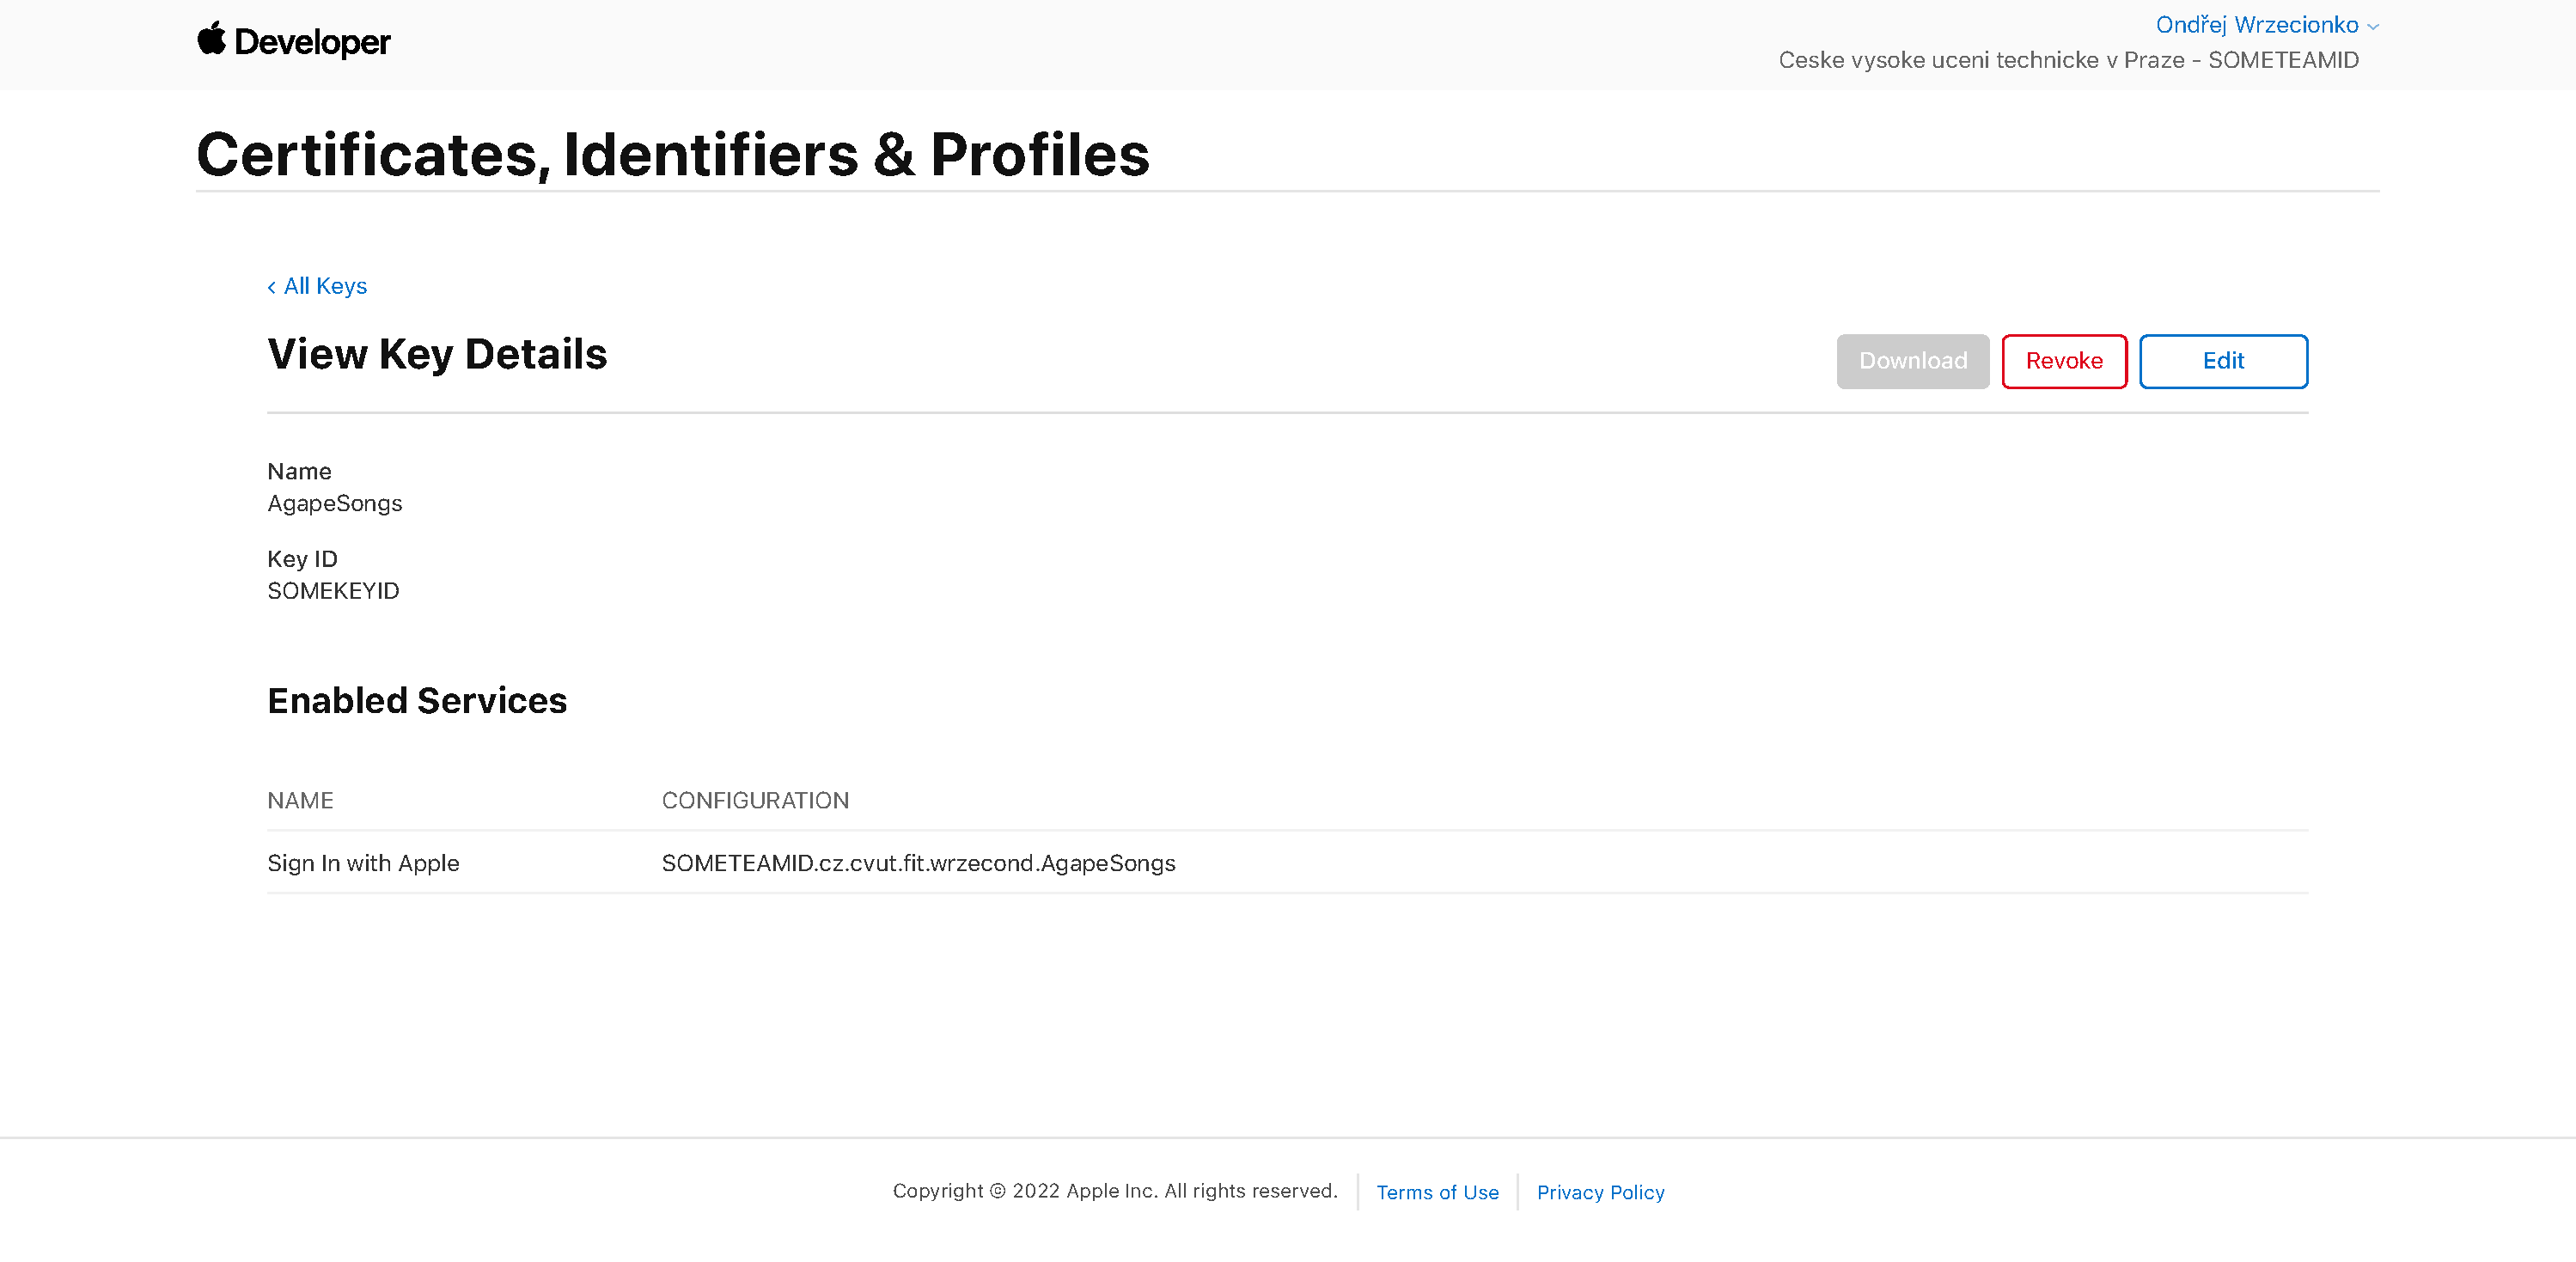
\includegraphics[width=\textwidth]{images/4-implementace/4-1-prihlaseni-pres-apple-klic.pdf}
    \caption{Apple vývojářský portál -- nastavení klíče pro Přihlášení přes Apple}
\end{figure}

Jak klíč, tak identifikátor aplikace nastavuji v konfiguračním souboru serveru, což je v případě frameworku Spring Web soubor \texttt{application.properties}, který je umístěn ve stejné složce jako výsledný server.

\begin{listing}[H]
\begin{minted}[breaklines,breaksymbolleft=]{properties}
auth.keyPath=/root/server/key.p8
auth.keyId=SOMEKEYID
auth.teamId=SOMETEAMID
\end{minted}
\caption{Ukázka konfiguračního souboru serveru \texttt{application.properties}}
\end{listing}

\begin{listing}[H]
\begin{minted}[breaklines,breaksymbolleft=]{kotlin}
// AuthService.kt
private fun appleAuth (code: String) : AppleUserInfo = tryCatch {
    val body  = networkService.appleAuthRequest(code, generateJWT())
    val token = Gson().fromJson(body, AppleToken::class.java)
    val payload = token.id_token.split(".")[1]
    val decoded = String(Decoders.BASE64.decode(payload))
    Gson().fromJson(decoded, AppleUserInfo::class.java)
}

private fun generateJWT () = Jwts.builder()
    .setHeaderParam(JwsHeader.KEY_ID, keyId)
    .setIssuer(teamId)
    .setAudience(APPLE_ENDPOINT)
    .setSubject(CLIENT_ID)
    // valid for 300 seconds
    .setExpiration(Date(300 * 1000 + System.currentTimeMillis()))
    .setIssuedAt(Date(System.currentTimeMillis()))
    .signWith(loadKeyFromFile(), SignatureAlgorithm.ES256)
    .compact()

// NetworkService.kt
@Service
class NetworkService {
    // Initiate HTTP client for network requests
    private val client = HttpClient(Java) {
        install(JsonFeature) {
            serializer = GsonSerializer {}
        }
    }

    fun appleAuthRequest (code: String, secret: String) : String = runBlocking {
        client.submitForm<HttpStatement>(
            url = AuthService.APPLE_ENDPOINT + AuthService.APPLE_PATH,
            formParameters = Parameters.build {
                append("client_id", AuthService.CLIENT_ID)
                append("client_secret", secret)
                append("grant_type", "authorization_code")
                append("code", code)
            }
        ).execute().receive()
    }
}
\end{minted}
\caption[Ukázka Service pro připojení k Apple serveru]{Třída \texttt{AuthService} při požadavku o přihlášení přes Apple vygeneruje JSON web token, který předá spolu s obdrženým kódem třídě  \texttt{NetworkService} komunikující s Apple serverem. Ta pak provede HTTP požadavek a vrátí informace o přihlášeném uživateli, které \texttt{AuthService} zpracuje a převede na informace o přihlášeném uživateli}
\end{listing}
